% APJ Reference: http://aas.org/journals/authors/common_instruct#_Toc2

\documentclass[iop]{emulateapj}
% \documentclass[12pt,preprint]{aastex}


% Define the sun symbol for use with solar mass
% \newcommand{\Sun}{\odot}
\newcommand{\vect}[1]{\boldsymbol{#1}}
% \usepackage{amssymb}
%\usepackage{xfrac}
% \usepackage{amsmath}
% \usepackage{multirow}
% \usepackage{array}
% \usepackage[lofdepth,lotdepth]{subfig}
%\usepackage{todonotes}

%\newcommand{\TODO}[1]{\todo[inline]{#1}}
\usepackage{float}
\usepackage{natbib}

% \newcolumntype{x}[1]{%
% >{\centering\hspace{0pt}}p{#1}}%


\bibliographystyle{apj}

\shortauthors{Brenner}
\shorttitle{Characterizing stellar phenomena with fractals and multifractals}

%--------------------
%	Begin document
%--------------------
\begin{document}
%
\title{Fractal and Multifractal Analysis as Tools to Characterize Supernovae and Molecular Clouds}
%
\author{Samuel Brenner\altaffilmark{1}}
\email{samuel.e.brenner@gmail.com}
%\author{Tomasz Plewa\altaffilmark{1}}
%\email{tplewa@fsu.edu}
%
%\author{Andrzej Odrzwolek\altaffilmark{2}}
%\email{andrzej's email}
%
\altaffiltext{1}{Young Scholars Program, Florida State University}
%
%
%
%--------------------
%	Begin Abstract
%--------------------
\begin{abstract}
\textit{copy-pasted from discussion for now} New opening...

In Sect. \ref{Results}, we found the fractal dimension of the flame front in a Type Ia supernova to be 1.05, which is at least 0.25 lower than the values given in the literature. One possible cause for the discrepancy between the fractal dimension of the flame front found here and the values provided is the relative coarseness of the model used. More importantly, the model used has been calculated in two dimensions, so it cannot fully account for the characteristics of three-dimensional turbulence. Regardless of these shortcomings, we developed a robust implementation of fractal analysis that can investigate this discrepancy further. In addition, this implementation has the ability to process simulation results obtained with or without uniform meshes.
 
We found that the multifractal spectra of the molecular cloud become wider over the course of the cloud's evolution. This can be explained as follows: as the system evolves, it transitions from a homogeneous cloud-like morphology to a more varied structure that eventually contains both overdense regions and regions of much lower densities than were originally present. In addition, the fractal dimension of the entire structure decreases from a little less than 3 (where the structure is primarily sheet-like) to $\approx 2.7$ (in the intermediate state) to $\approx 1.7$ (when the collapsed filaments have formed).

Future investigations will focus on the 
\end{abstract}
%
%
%
%--------------------
%	Begin keywords
%--------------------
\keywords{supernovae, fractals, multifractals}
%
%
%
%--------------------
%	Begin Body
%--------------------

\section{Introduction}
Many physical phenomena cannot be characterized by the idealizations of Euclidean geometry alone; they exhibit ``roughness'' of morphology. That is, they have a detailed structure at any arbitrarily small size scale \citep[see][]{Falconer2003}. We can quantify this roughness with the concept of a fractal dimension, which---just like the Euclidean dimension---tells how some figure fills a space, so that a rougher figure would tend to have a higher fractal dimension than a smooth one. Multifractal analysis extends this paradigm of a fractal dimension by permitting us to examine how those fractal characteristics themselves change with scale; in fact, they may even be fractal themselves. In this paper, we detail the application of fractal geometry to flame fronts in exploding white dwarfs and then analyze the multifractal characteristics of star-forming molecular clouds.

\subsection{Fractal analysis of Type Ia supernova flame fronts}
The accepted model for a Type Ia supernova is a white dwarf that accumulates mass from a binary companion until it reaches a mass so large that the compression and heating of the core causes heavier elements to begin fusing. This fusion gives off even more heat, starting a cascade of fusion reactions: a subsonic thermonuclear flame front. This front spreads rapidly throughout the star and causes the explosion of the white dwarf.

The morphology of the expanding flame front can be dramatically affected by multiple types of perturbations. \cite{Landau1959} showed that the flame surface is subject to Landau-Darrieus instability in which the front is convoluted due to thermal expansion across the flame front. It is also widely established \citep{Khokhlov} that Rayleigh-Taylor instability, in which a denser fluid pushes through a less-dense one under the influence of a gravitational field, can contort the deflagration front in a supernova. These wrinkles on the surface of the flame front increase the front's effective surface area, and because the flame speed is proportional to the flame's surface area, the convolution of the surface can influence the rate at which the flame consumes the stellar material. Thus, characterizing the shape of the flame front plays a crucial part in characterizing the supernova explosion process as a whole.

\begin{figure}[ht]
	\begin{center}
	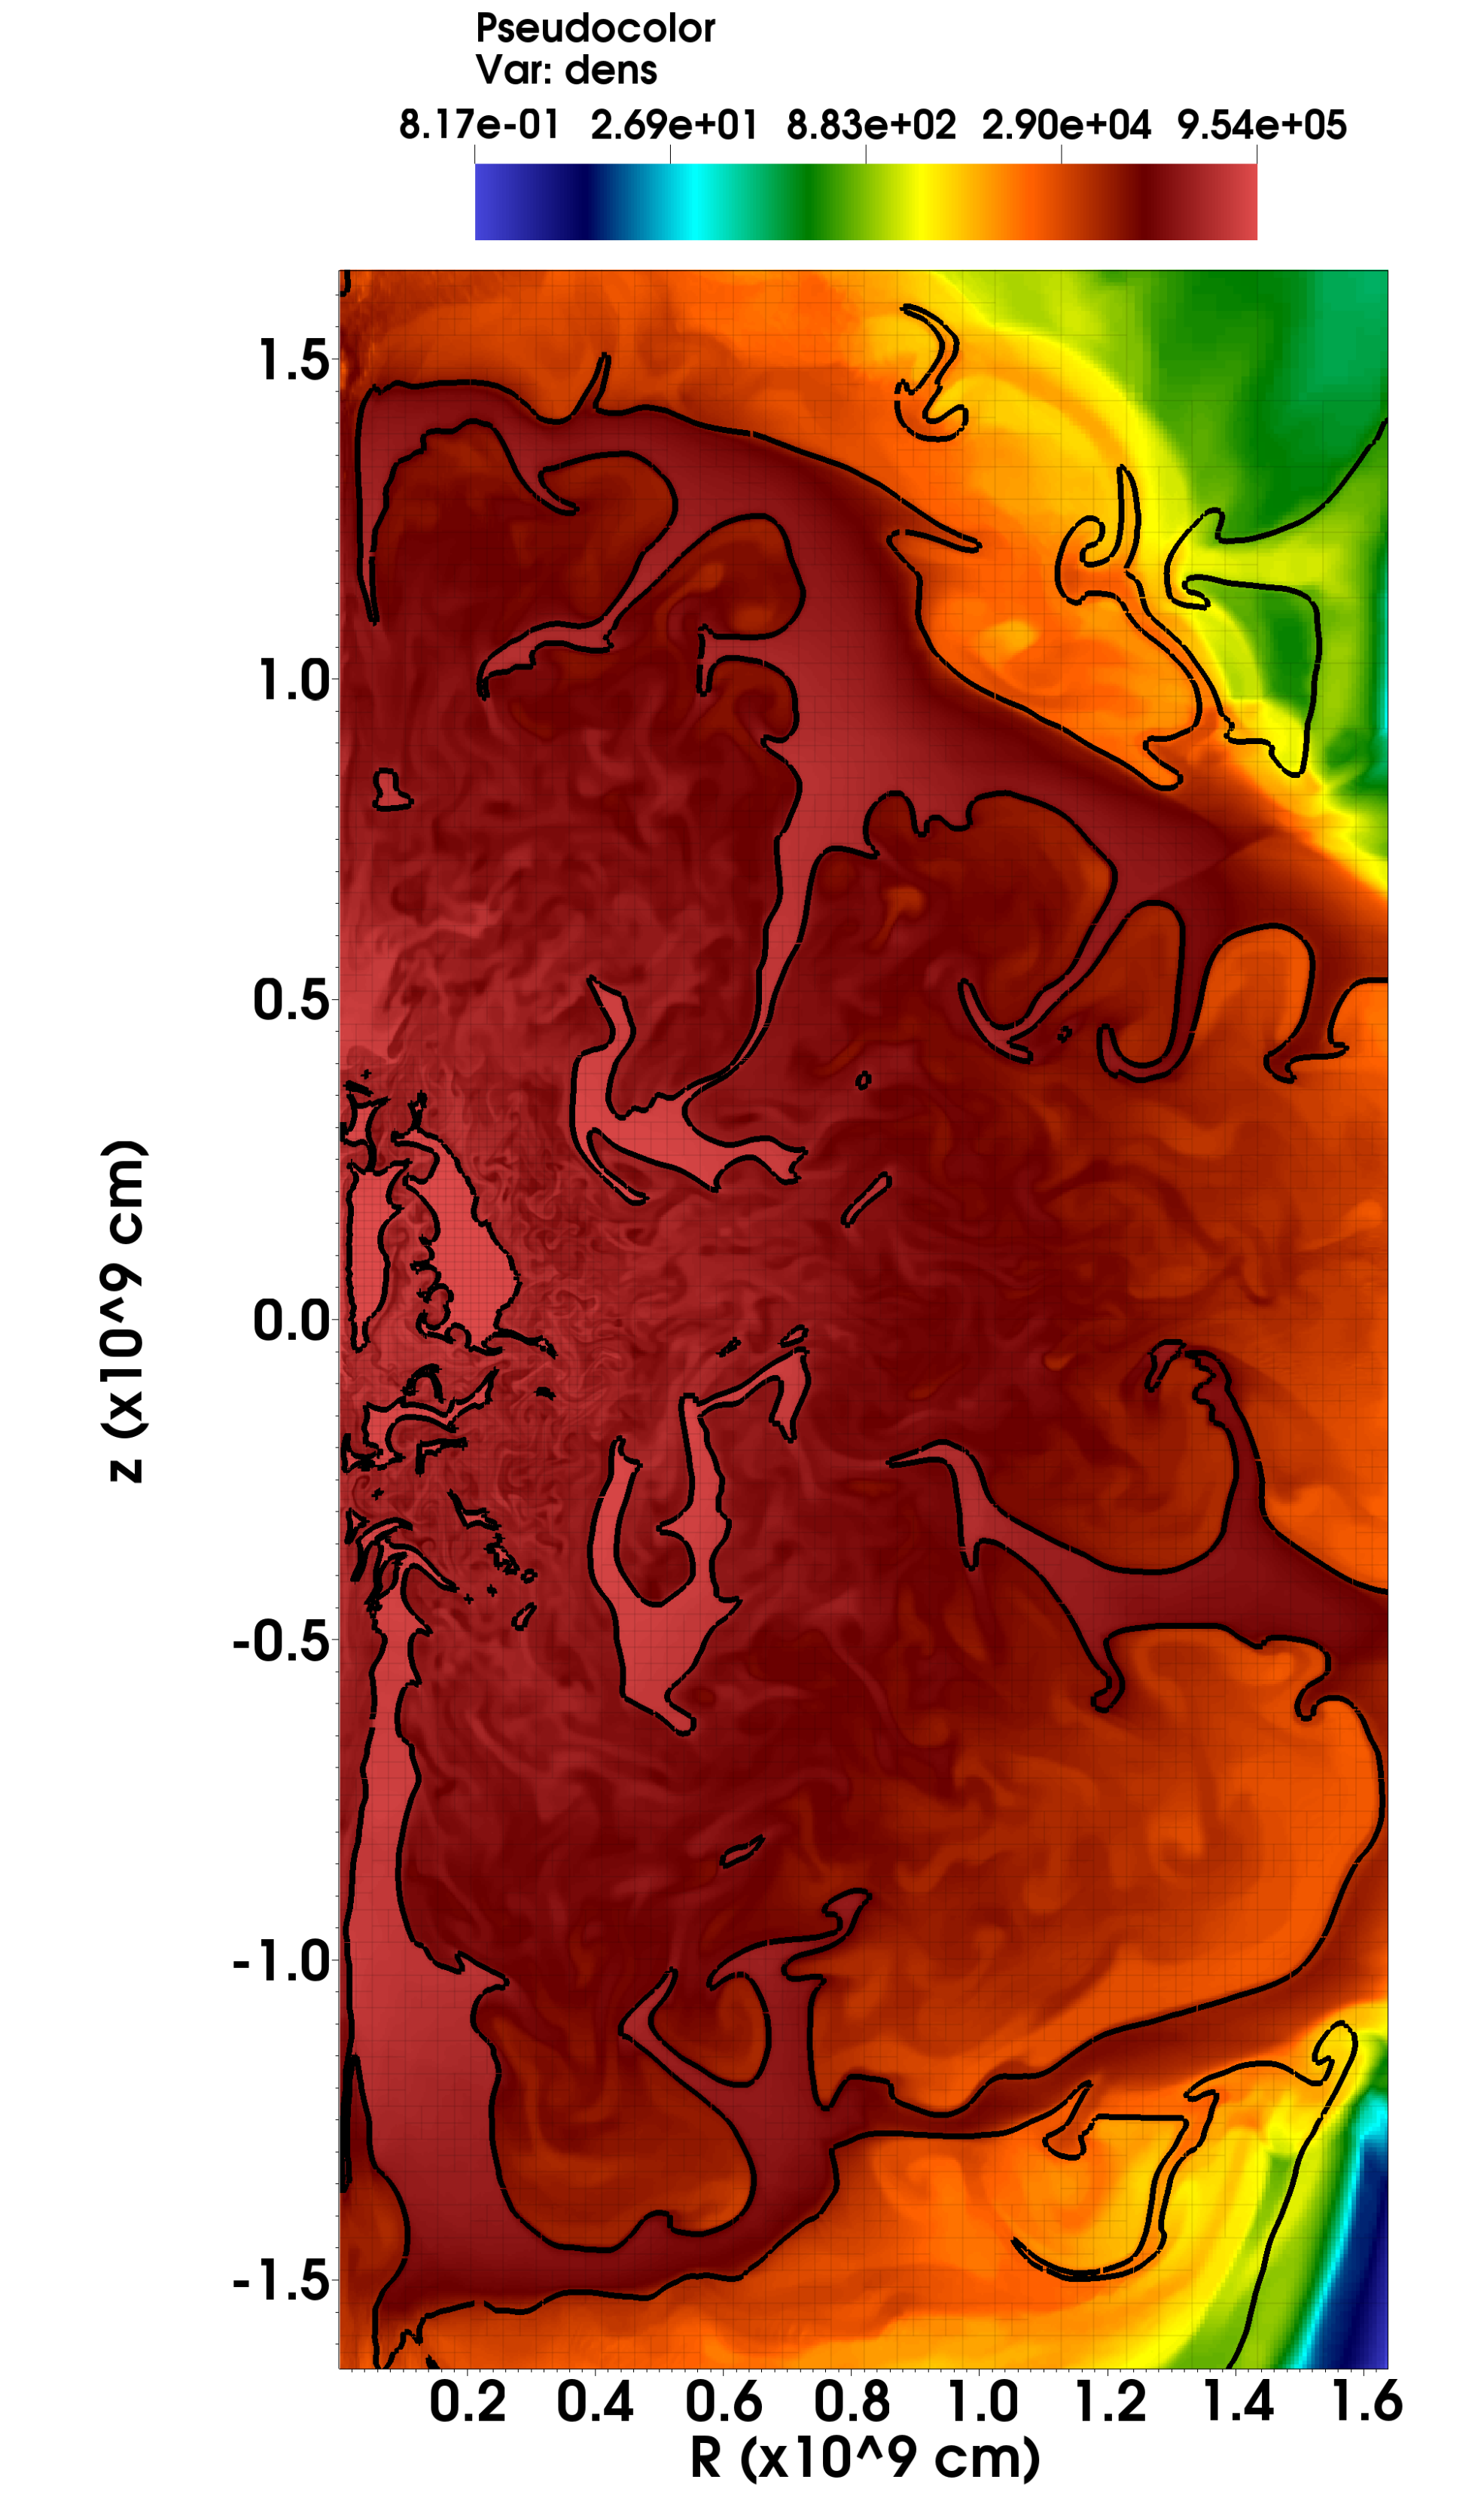
\includegraphics[width=0.35\textwidth,clip=true]{Graphics/n7d1r10t15b0011_cropped.png}
	\caption{Model of a Type Ia supernova in cylindrical coordinates where $z$ is the axis of symmetry. False color shows density in $\mathrm{g/cm^3}$. The contour of the flame front is shown with the black line. Thin grey lines show outline of mesh structure used in model.
	\label{f:flamefrontwithcontour}}
	\end{center}
	\end{figure} 

The convolutions of the surface of a turbulent front can be viewed within the framework of fractal geometry, as was proposed by \cite{Mandelbrot1975} and further developed by \cite{Timmes1994}. In particular, Timmes showed that the final effective speed $v_{eff}$ of the flame front can be expressed as a function of its fractal dimension:
\begin{equation} 
	v_{eff} = v_{lam} \left(\frac{l_{min}}{l_{max}}\right)^{2 - D},
\end{equation}
where $v_{lam}$ is the laminar flame speed (that is, the speed of the flame in the absence of perturbations), $l_{min}$ is the minimum length scale at which the turbulence takes place, $l_{max}$ is the maximum length scale at which the turbulence takes place, and $ D $ is the fractal dimension of the flame front.

In Sect. \ref{Methods}, we discuss the implemention of a method to perform fractal analysis of a supernova flame front. The results are discussed in Sect. \ref{Results}, and the implications of our findings are discussed in Sect. \ref{Discussion}.

\subsection{Multifractal analysis of star-forming molecular clouds}
Clouds often form in the interstellar medium (ISM), and turbulence like that caused by stellar winds can create structures which under their own gravity collapse. \citep{Bergin2007}. The densest parts of these collapsed regions are protostars that eventually begin to undergo fusion and become evolved star systems. 

Star-forming molecular clouds have been observed to follow a general progression of morphology over time \citep[see][for example]{Shu1987}. A somewhat uniform cloud of gas first coalesce into sheet-like structures under the influence of some external perturbation, which then collapse under their own gravity to form filament-like structures. Further self-gravitation causes blobs \footnote{Is there a more specific way to say this? I mean to say something like ``spheres'', but I know they're not spherical. ``Points'' is misleading, too.} of high relative density to form within these filaments, which we recognize as protostars.

The structure of the star-forming cloud at any time can be quantified by the spectrum of multifractal dimensions, which indicates the abundance of substructures with a given density. Thus we can quantitatively indicate how uniformly filament-, sheet-, or space-like any structure is. Figure \ref{f:cloudevolution} depicts the evolution of one of these molecular clouds.

In Sect. \ref{Methods}, we discuss the implemention of a method to determine the multifractal spectrum of these star-forming clouds. The results are discussed in Sect. \ref{Results}, and the implications of our findings are discussed in Sect. \ref{Discussion}.

\begin{figure*}[ht]
	\begin{center}
	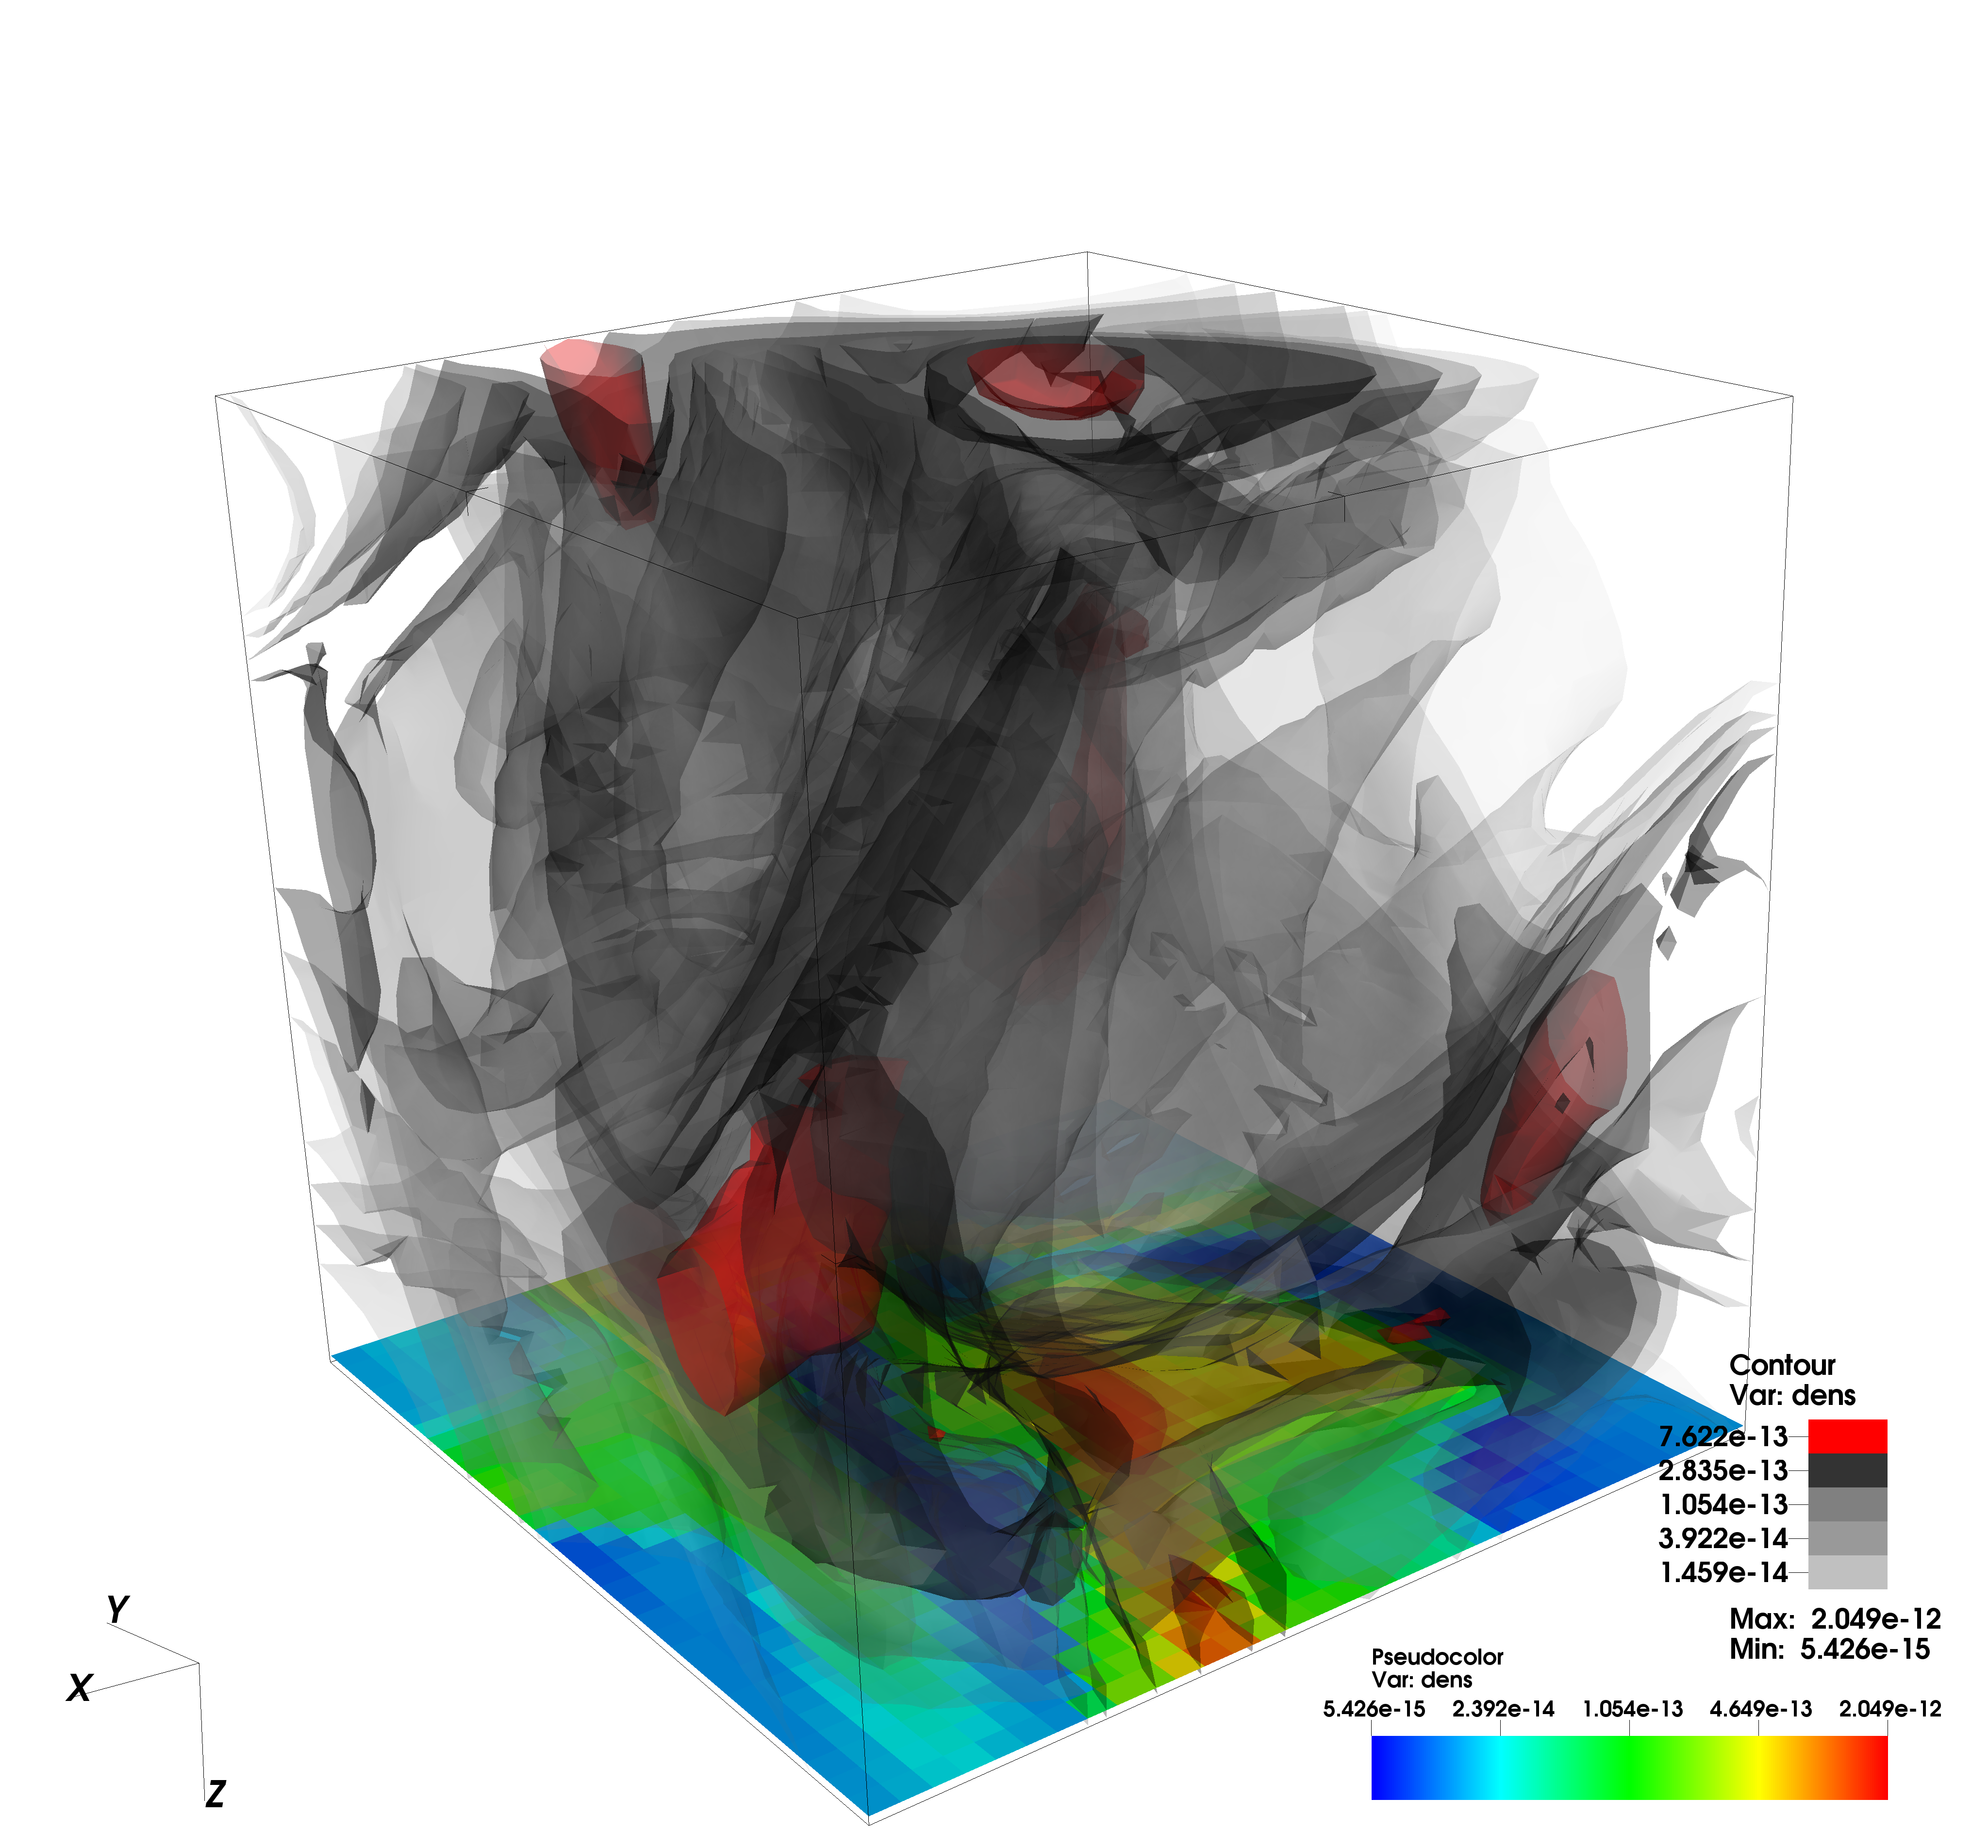
\includegraphics[height=5.5cm,clip=true]{Graphics/bbb_0375_dens_contour_00500000.png}%
	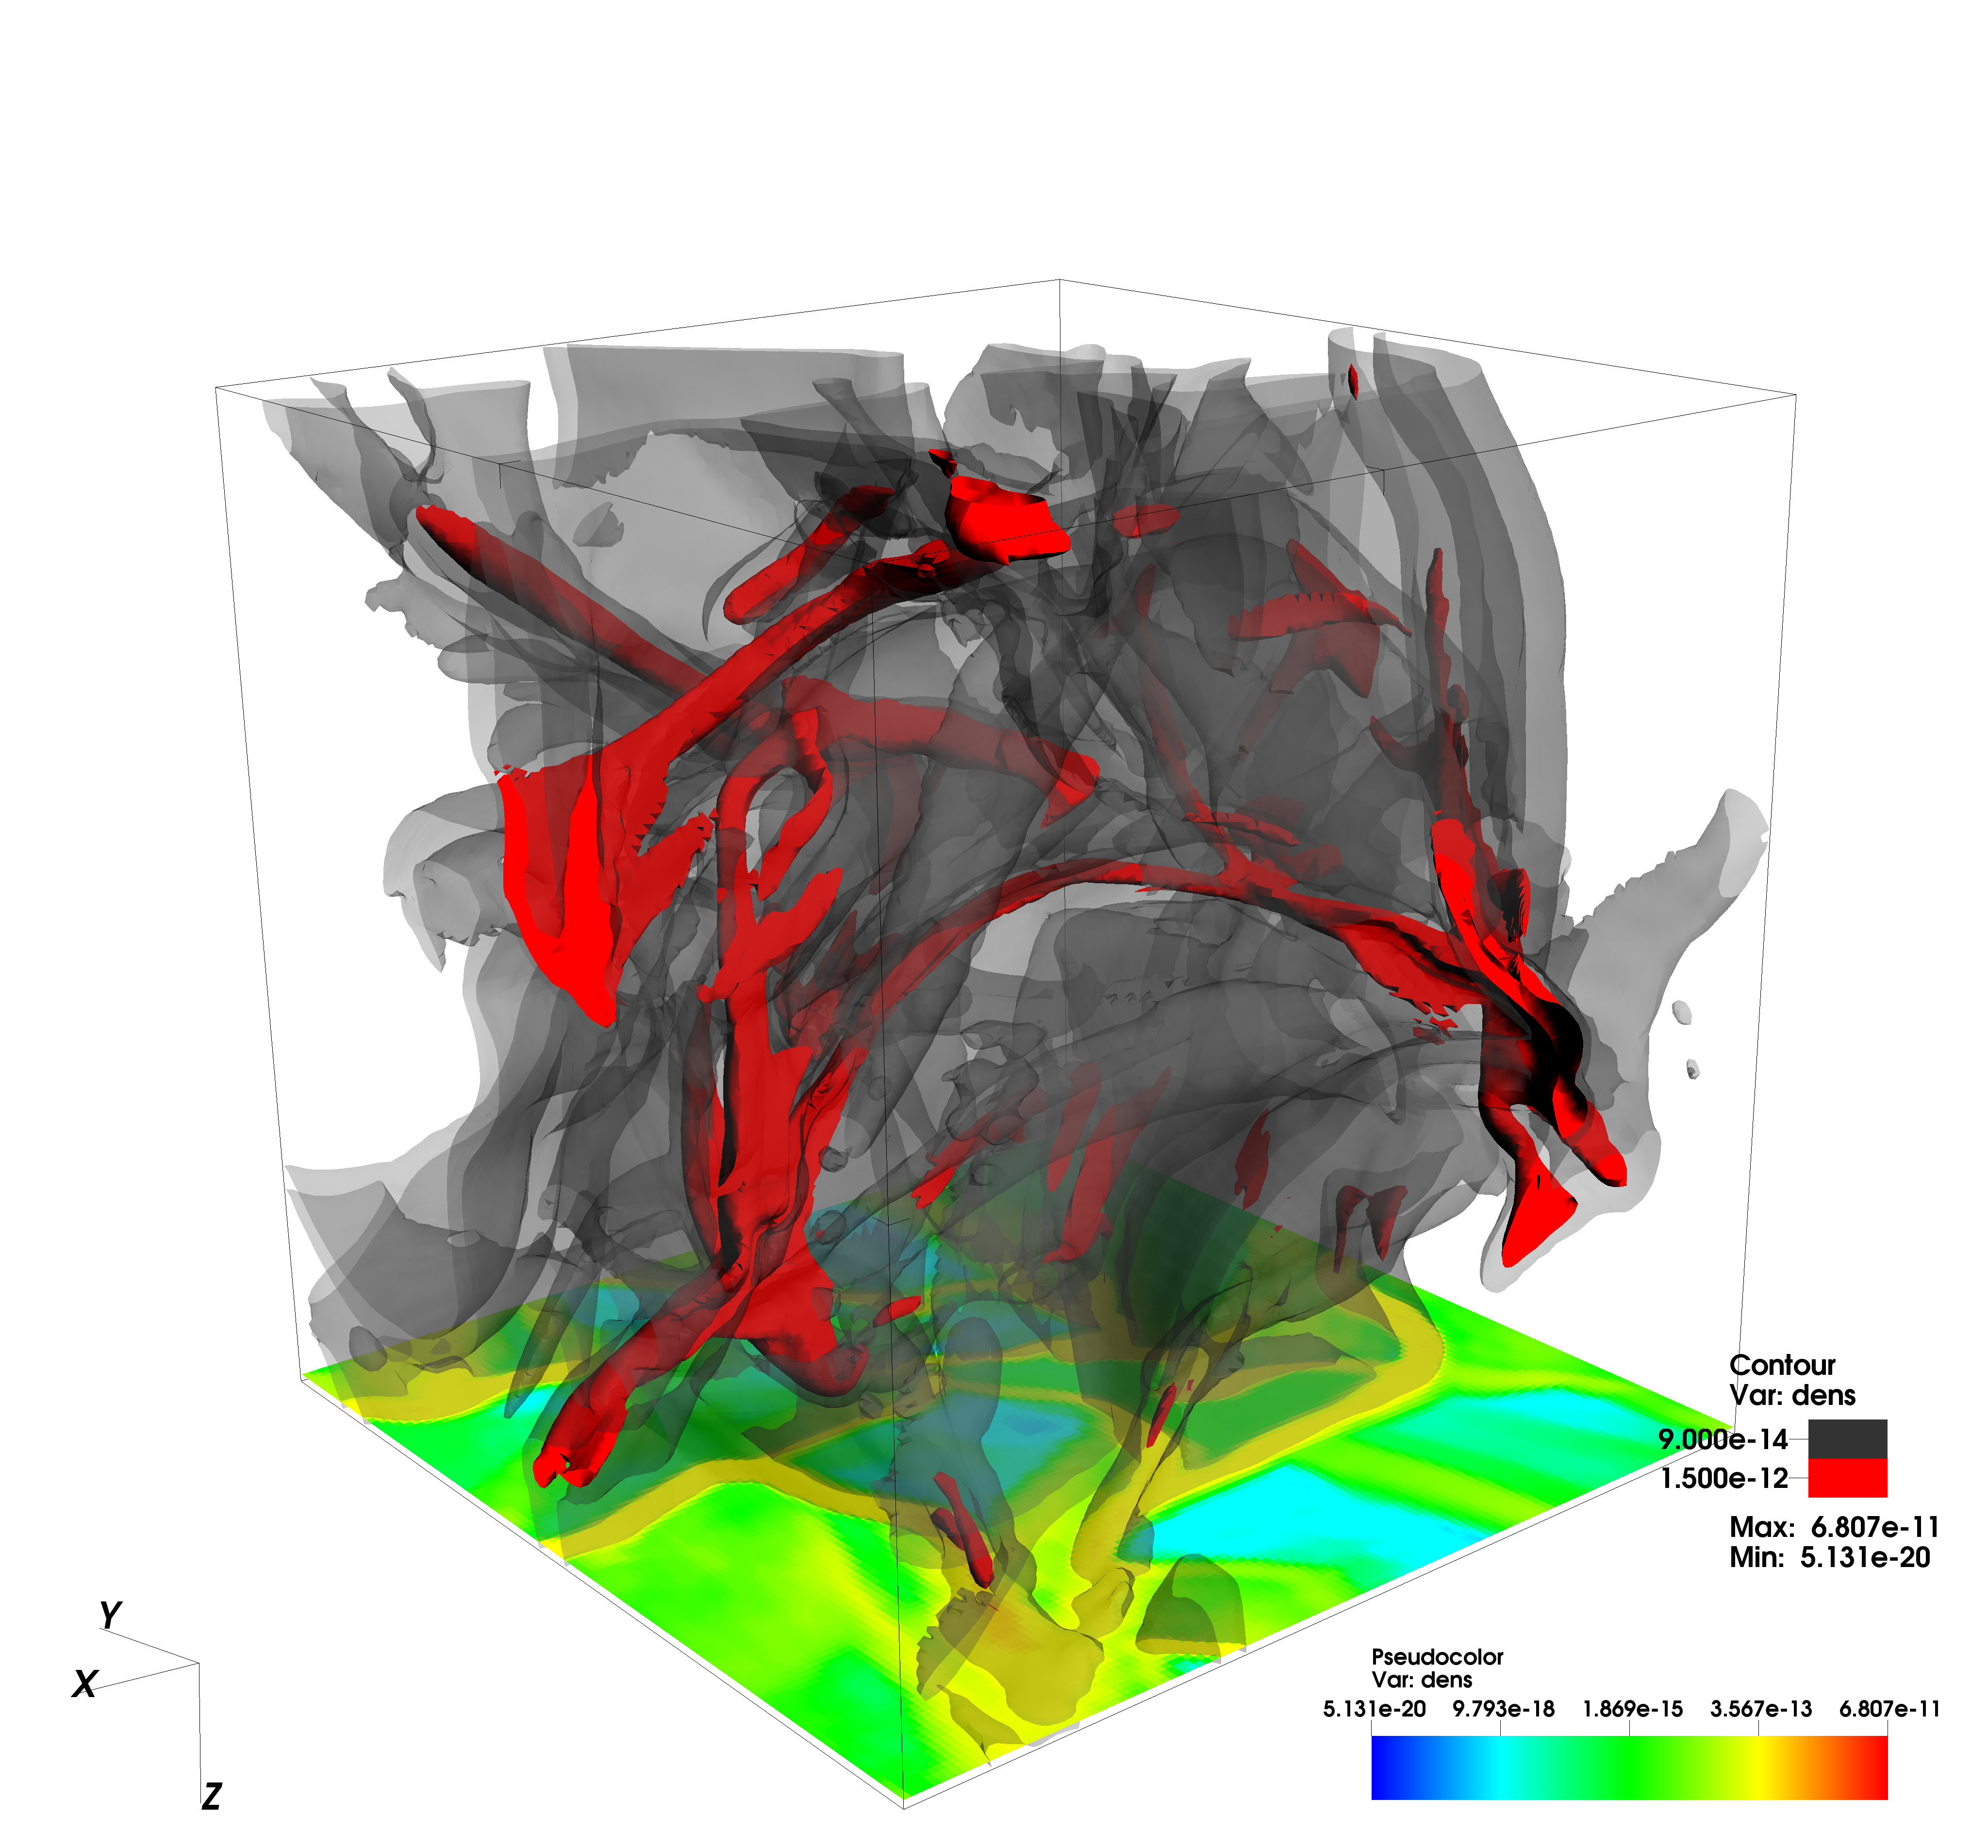
\includegraphics[height=5.5cm,clip=true]{Graphics/bbb_0375_dens_contour_0200_0002.png}%
	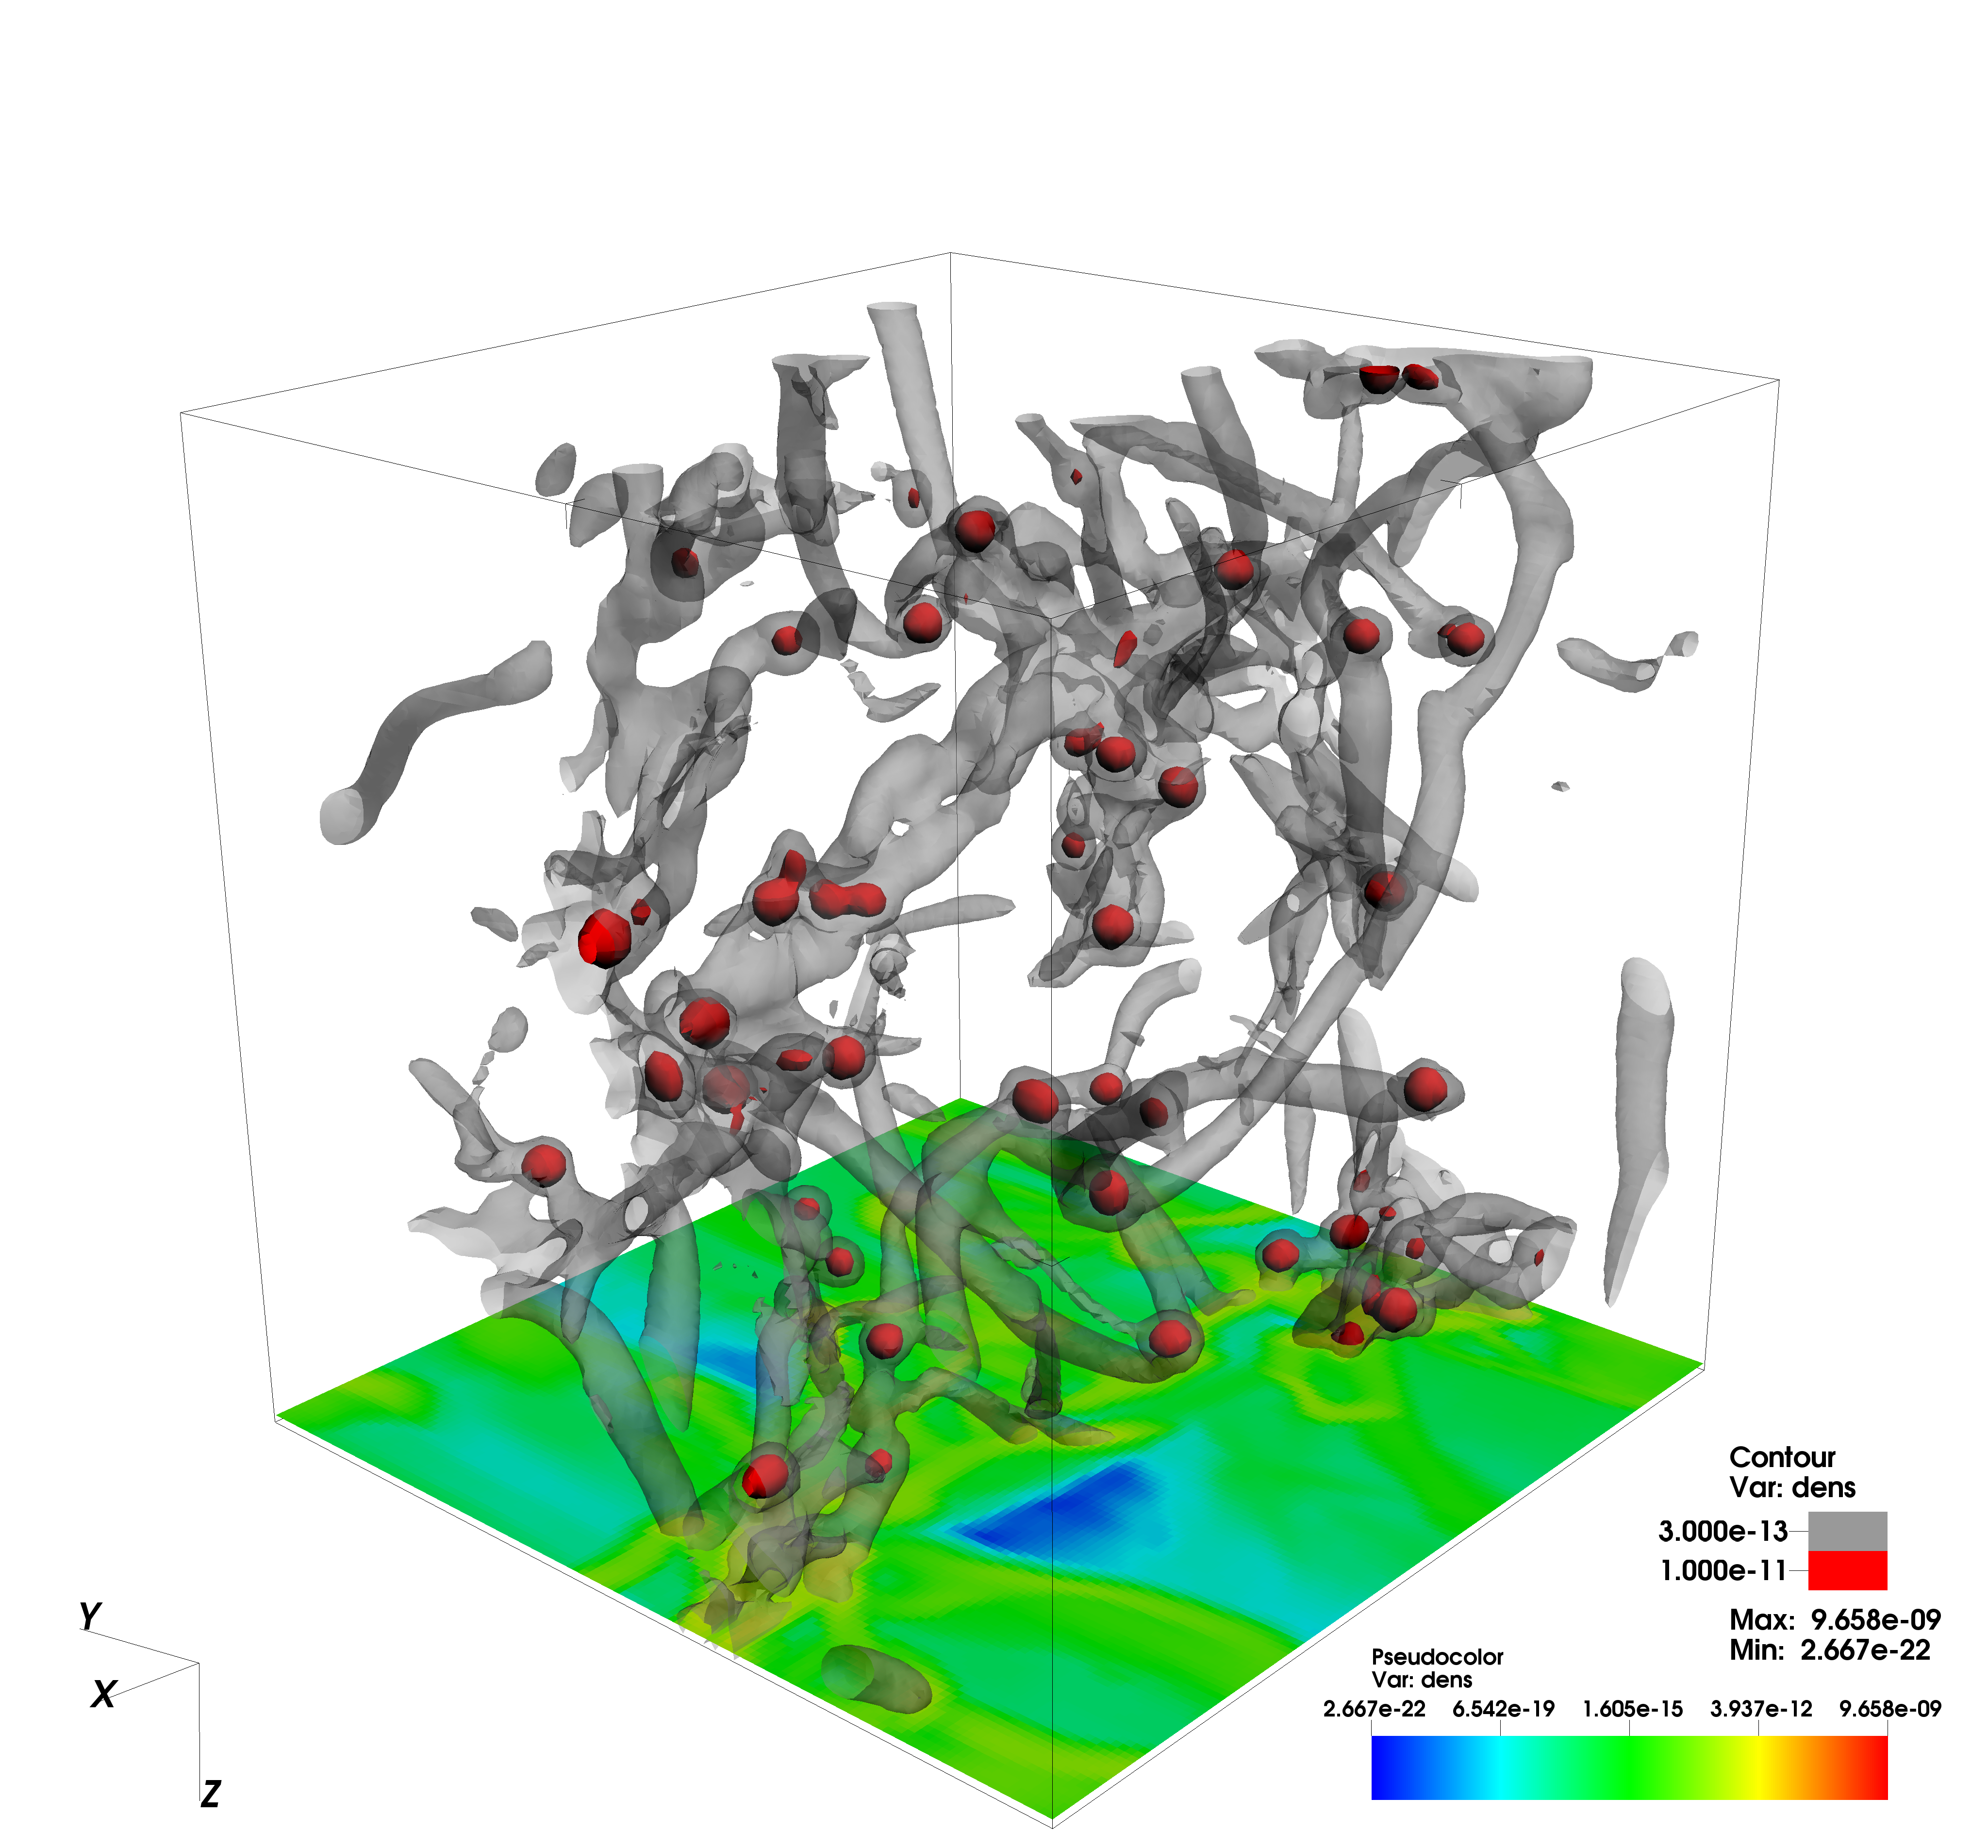
\includegraphics[height=5.5cm,clip=true]{Graphics/bbb_0375_dens_contour0000.png}
	\end{center}
	\caption{Evolution of density contour in a star-forming molecular cloud over time. The leftmost panel shows the density contour at early times, with sheet-like structures most prominent. The middle panel shows the collapse of those sheets into filaments in the densest (red) regions at intermediate times. The rightmost panel shows a near-complete transition to filaments, and the densest (red) regions indicate the position of protostars.}
	\label{f:cloudevolution}
	\end{figure*}






\section{Methods}\label{Methods}

\subsection{Fractal analysis methods}\label{FractalMethods}
A box-counting algorithm \citep[see][for example]{Falconer2003} was implemented in order to determine the fractal dimension of the flame front. With this algorithm we can describe the fractal dimension, $\mathrm{dim}$, as
\begin{equation}\label{dimensioneqn}
	\mathrm{dim}_B = \lim_{\epsilon \to 0} \frac{\log N(\epsilon)}{\log (1 / \epsilon)},
\end{equation}
where $N$ is the number of boxes containing the structure of interest.  To implement the estimation in Eq. \ref{dimensioneqn}, one must introduce coarse-graining of the data under study. In the flame front analysis performed here, trilinear interpolation is performed in order to determine the location of the flame front within the coarse mesh. For each level of coarse-graining, $\log{N(\epsilon)}$ and $\log{(1/\epsilon)}$ is calculated, and a linear regression is performed on the four points with finest resolution in order to estimate the dimension as given in Eq. \ref{dimensioneqn}.

\subsection{Multifractal analysis methods}\label{MultifractalMethods}
The multifractal spectrum of some set is the plot of $f(\alpha)$ vs. $\alpha$, where $f(\alpha)$ is the fractal dimension of the subset of all points with local density $\alpha$ \citep[see][for example]{Falconer2003}. To obtain the multifracta spectra we use the method of \cite{Chhabra1989}. We reparametrize both $f$ and $\alpha$ as functions of a moment exponent $q$ that serves to weight the features of the density on various scales. For every value of $q$, we define the normalized measure $\mu_i(q, \epsilon)$ of box $i$ with side length $\epsilon$ as
\begin{equation} 
	\mu_i(q, \epsilon) = \frac{[M_i(\epsilon)]^q}{\sum_j[M_j(\epsilon)]^q},
\end{equation}
where $M_i$ is the mass contained in each box $i$. Now we can express $f(\alpha)$ as
\begin{equation}
	f(q) = \lim_{\epsilon \to 0} \frac{\sum_i \mu_i(q, \epsilon) \log[\mu_i(q, \epsilon)]}{\log \epsilon},
\end{equation}
and $\alpha$ as
\begin{equation}
	\alpha (q) = \lim_{\epsilon \to 0} \frac{\sum_i \mu_i(q, \epsilon) \log[M_i(\epsilon)]}{\log \epsilon}.
\end{equation}


\subsection{Verification}\label{Verification}

Our implementation of the box-counting algorithm was verified against computer-generated data with known fractal characteristics. The implementation was able to recover the theoretical dimension with 12\% accuracy on average, as can be seen in Table~\ref{t:table}. Our implementation of the multifractal algorithm was verified against a computer-generated multifractal system and produced the expected plot of $f(\alpha)$ vs. $\alpha$ as can be seen in Fig. \ref{f:cantorset}. 

\begin{figure*}[ht]
	\begin{center}
	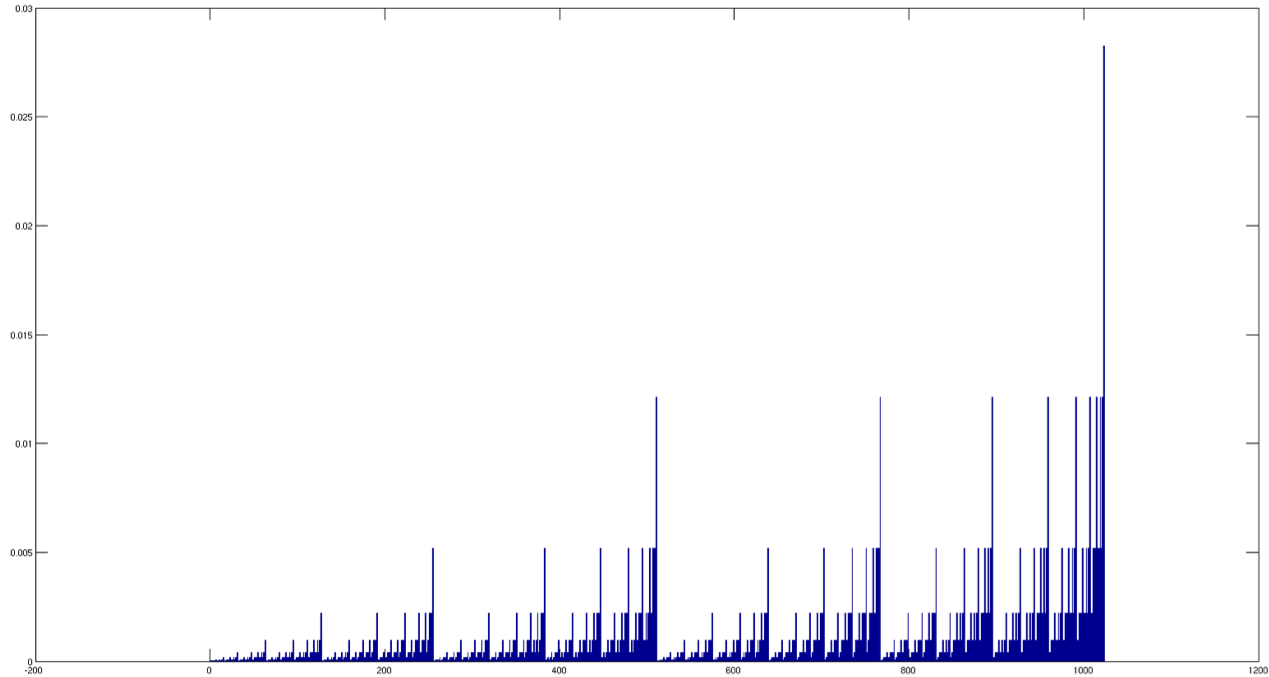
\includegraphics[height=4cm,clip=true]{Graphics/binomialcantor1024.png}%
	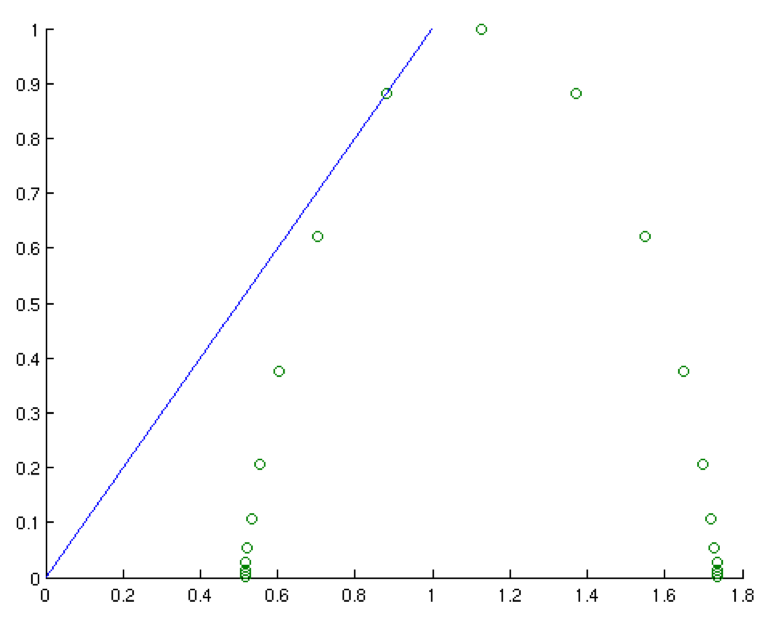
\includegraphics[height=4cm,clip=true]{Graphics/firstf(a)plot!.png}%
	\end{center}
	\caption{The one-dimensional binomial Cantor set (left) and the multifractal spectrum produced by our implementation in the process of verification. The obtained results match predictions: the maximum value of $f(\alpha)$ is $1$ (which indicates that the set as a whole has a dimension of one), the shape is parabolic (characteristic of plots of this set \citep{Chhabra1989}), and each plot intersects the blue line $f(\alpha) = \alpha$ (a characteristic of all multifractal spectra \citep{mandelbrotmultifractal})}
	\label{f:cantorset}
	\end{figure*}

\begin{table*}
\begin{center}
\caption{Theoretical vs. Calculated Fractal Dimensions Found in Fractal Analysis Validation}\label{t:table}
\begin{tabular}{lcccc}
Fractal Object 				&	Theoretical Dimension 	&	Calculated Dimension 	&	Error		&	Magnitude of percent error \\
\tableline\\
Dragon boundary				&	1.5236					&	1.487	                &	-0.037		&	2.4	\\
Vicsek Fractal (Box)		& 	1.4649					&	1.3264					&	-0.14		&	9.5	\\
Fibonacci Word				&	1.6379					&	1.45964					&	-0.18 		&	11	\\
Gosper Curve				&	2						&	1.72811					&	-0.27		&	14				\\
Boundary of Gosper Island	&	1.1292					&	1.2056					&	0.077		&	6.8	\\
Julia Set					&	2						&	1.49408					&	-0.51		&	25	\\
Julia $z^2+1/4$				&	1.0812					&	1.19677					&	0.12		&	11	\\
Levy C boundary				&	1.934					&	1.5656					&	-0.37		&	19	\\
Pythagoras Tree				&	2						&	1.74588					&	-0.25		&	13	\\
\tableline
\rule{0pt}{4ex}				&							&							& \textbf{Average: } & 12\\
\end{tabular}
\end{center}
\end{table*}


\section{Results}\label{Results}

\subsection{Fractal analysis}\label{FractalResults}
The box-counting method described in Sect. \ref{Methods} was applied to the contour shown in Fig. \ref{f:flamefrontwithcontour}. We found the fractal dimension of the contour to be 1.05, as can be seen in the plot of $\log N(\epsilon)$ vs. $\log (1 / \epsilon)$ in \ref{f:logNvsE}. \cite{Timmes1994} and \cite{Blinnikov1996} estimated the fractal dimension of flame fronts in three dimensions to be between 2.3 and 2.6. Intuitively, then, one would expect the fractal dimension of a flame front in two dimensions to be between 1.3 and 1.6, a discrepancy we examine in Sect. \ref{Discussion}.

\begin{figure}[ht]
	\begin{center}
	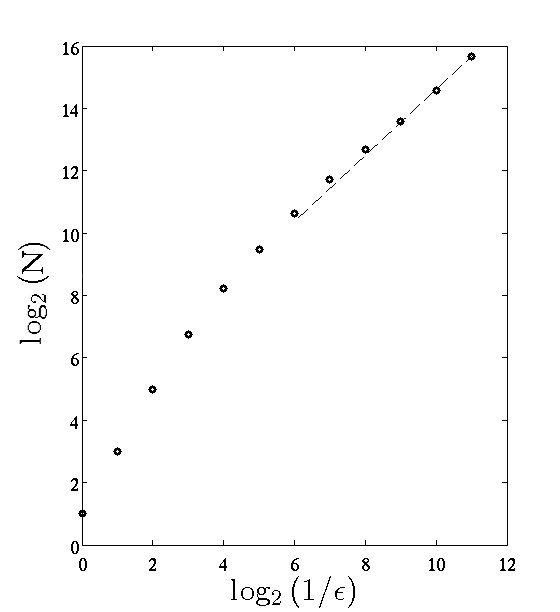
\includegraphics[width=0.37\textwidth,clip=true]{Graphics/logNvsE.png}
	\caption{Regression to find the fractal dimension of the flame contour shown in Fig. \ref{f:flamefrontwithcontour}. The slope of the regression line indicates the fractal dimension—about 1.05.
	\label{f:logNvsE}}
	\end{center}
	\end{figure} 


\subsection{Multifractal analysis}\label{MultifractalResults}

\begin{figure}[ht]
	\begin{center}
	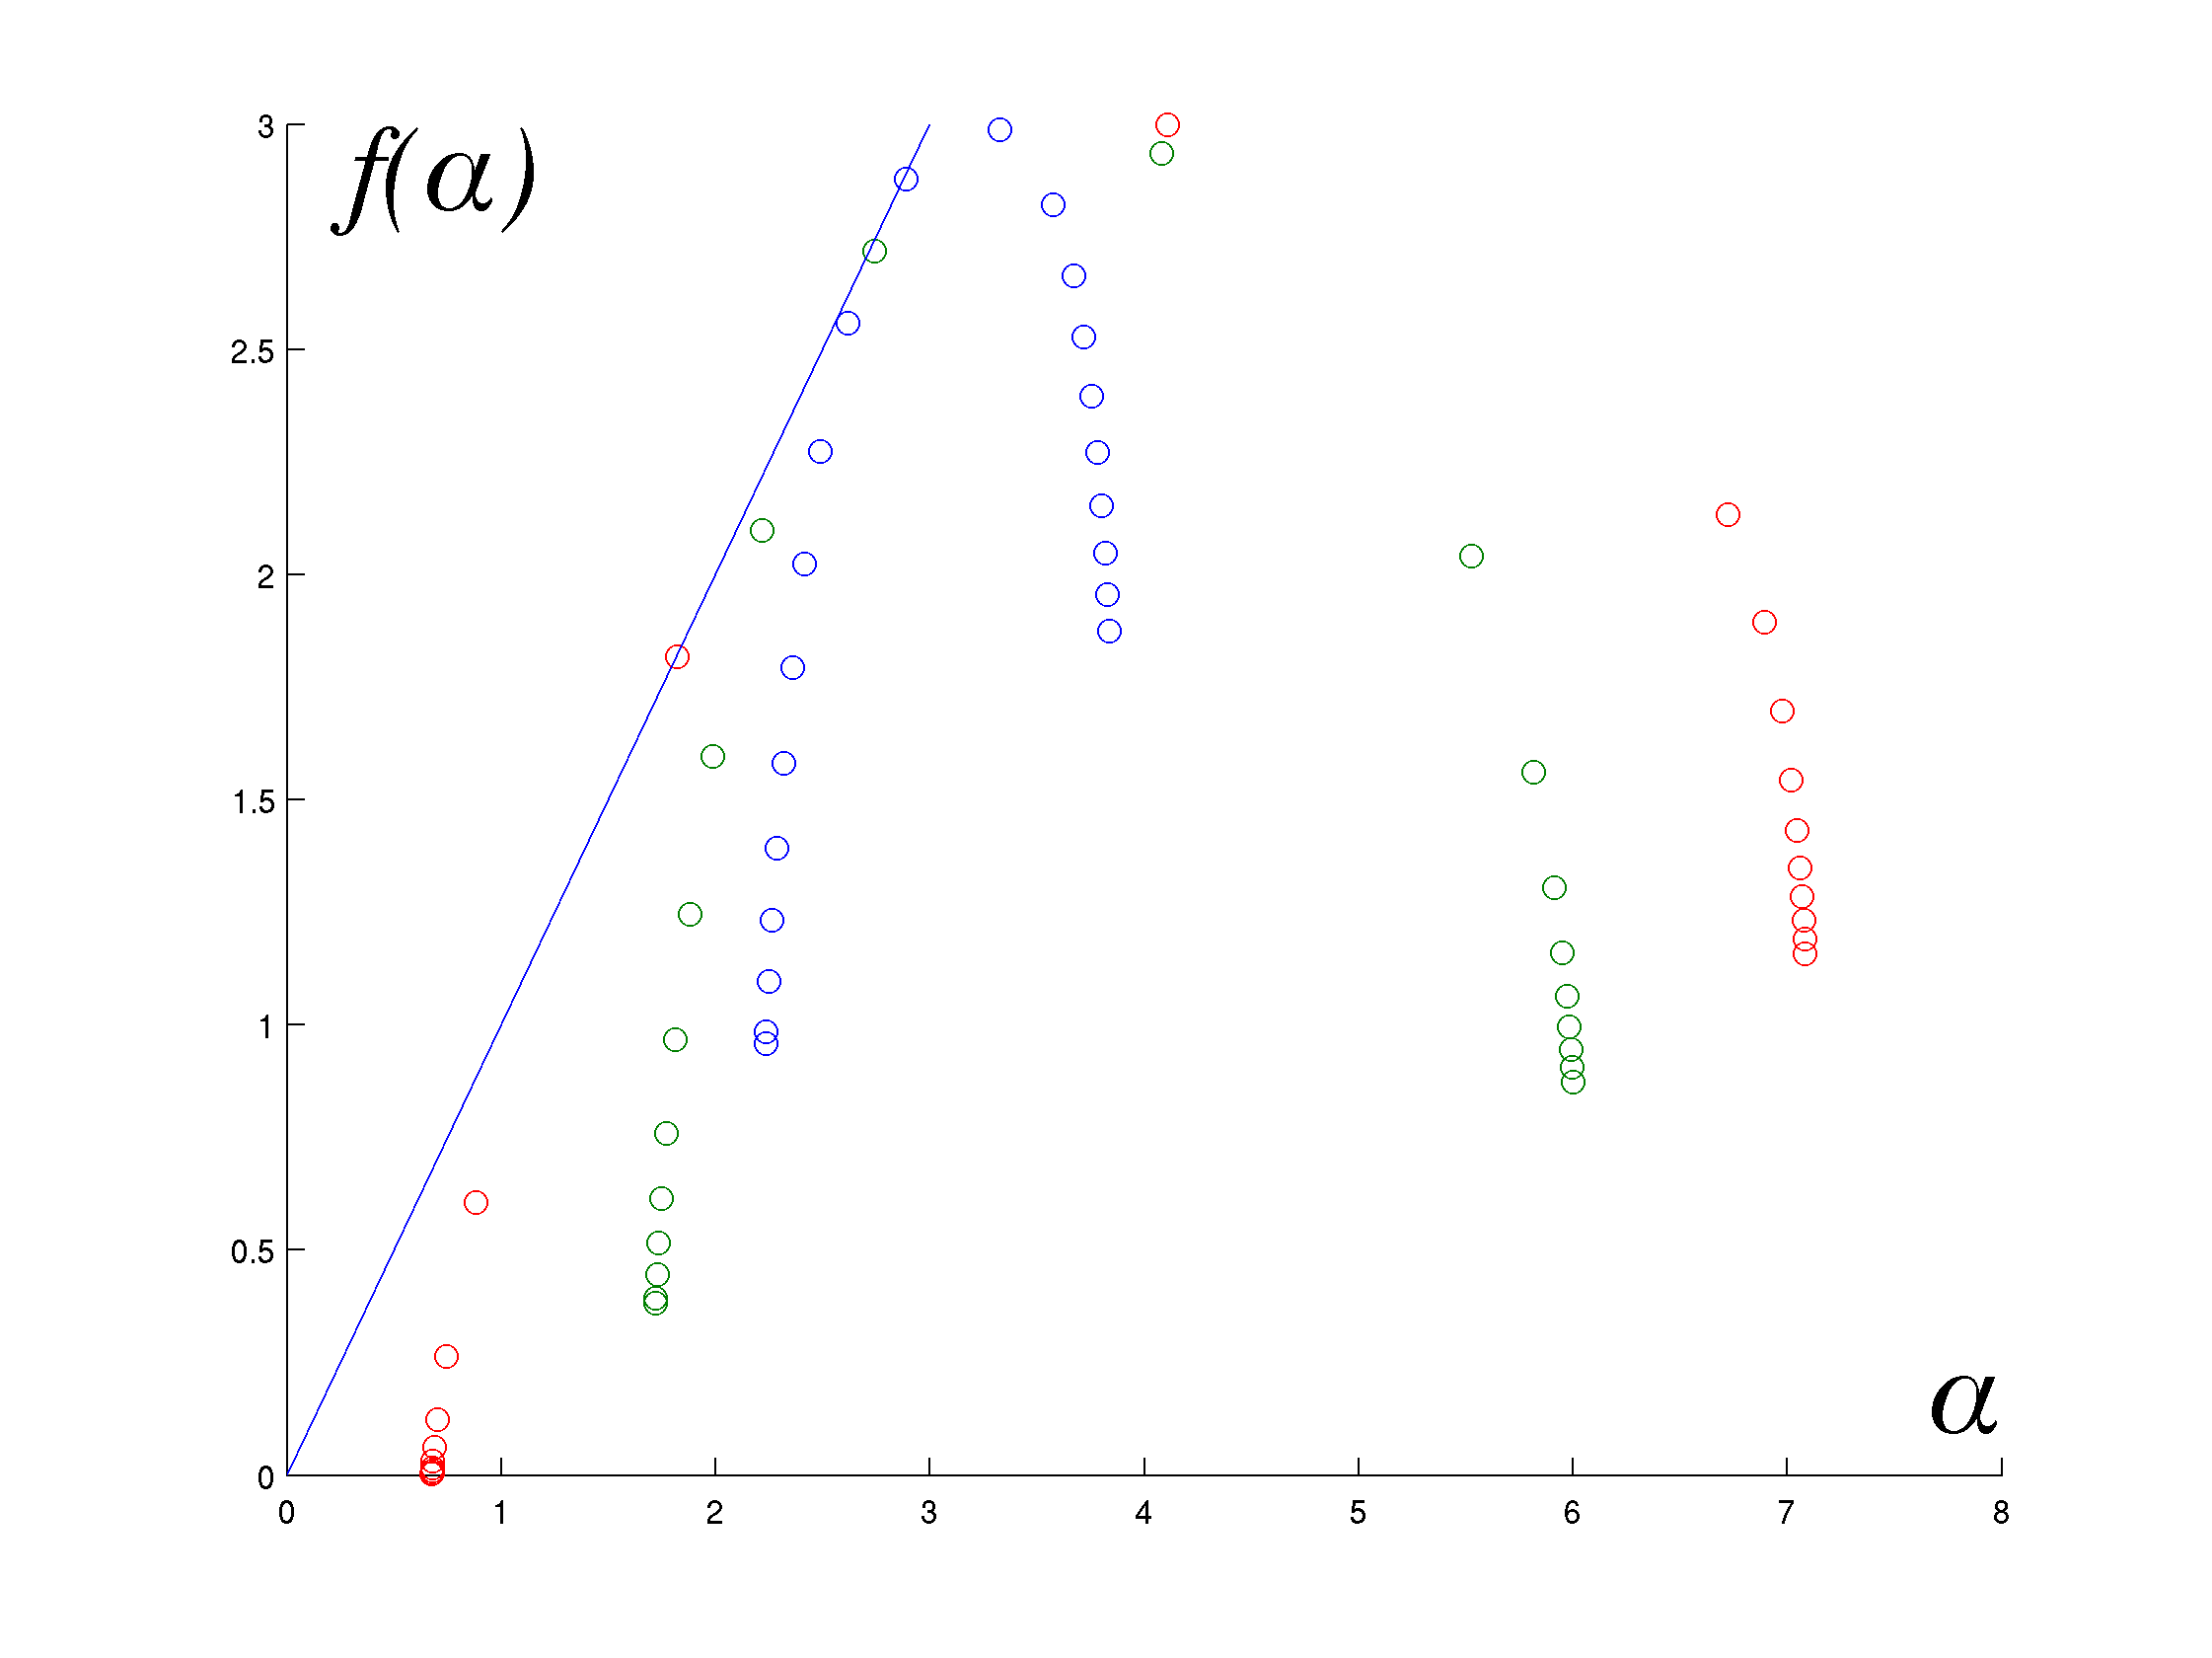
\includegraphics[width=0.45\textwidth,clip=true]{Graphics/falphaclouds.png}
	\caption{Plot of $f(\alpha)$ vs. $\alpha$ for the molecular cloud pictured in Fig. \ref{f:cloudevolution}. The blue curve shows the spectrum of the earliest timestep (corresponding to the leftmost panel of Fig. \ref{f:cloudevolution}); the green plot shows the spectrum of the middle timestep (middle panel of Fig. \ref{f:cloudevolution}); and the red plot shows the spectrum of the last timestep (rightmost panel of Fig. \ref{f:cloudevolution}). The blue line $f(\alpha) = \alpha $ intersects the curves at the points where $f(\alpha)$ gives the dimension of the entire structure.
	\label{f:falphamultifractal}}
	\end{center}
	\end{figure} 

The multifractal spectra generated from the molecular cloud pictured in Fig. \ref{f:cloudevolution} are presented in Fig. \ref{f:falphamultifractal}. The blue plot shows the spectrum of the earliest timestep (leftmost panel); the green plot shows the spectrum of the intermediate timestep (middle panel); and the red plot shows the spectrum of the last timestep (rightmost panel). The blue line, $f(\alpha) = \alpha $, intersects the curves at the points where $f(\alpha)$ gives the fractal dimension of the entire structure \citep{mandelbrotmultifractal}. Each curve has a maximum at $f(\alpha) \approx 3$, occurring when the moment exponent $q = 0$. This maximum, then, can be interpreted as the fractal dimension of the space in which the cloud lies \citep{Schroeder}. In the case of a molecular cloud in space, a dimension of 3 is to be expected. 

\section{Discussion}\label{Discussion}
In this work we constructed a tool allowing for fractal and multifractal analysis of simulation data on structured uniform and non-uniform meshes. We verified implementation for a number of fractal objects with known fractal properties, and applied our tool to select astrophysical problems. In particular, we examined the 

In Sect. \ref{Results}, we found the fractal dimension of the flame front in a Type Ia supernova to be 1.05, which is at least 0.25 lower than the values given in the literature. One possible cause for the discrepancy between the fractal dimension of the flame front found here and the values provided is the relative coarseness of the model used. More importantly, the model used has been calculated in two dimensions, so it cannot fully account for the characteristics of three-dimensional turbulence. Regardless of these shortcomings, we developed a robust implementation of fractal analysis that can investigate this discrepancy further. In addition, this implementation has the ability to process simulation results obtained with or without uniform meshes.
 
We found that the multifractal spectra of the molecular cloud become wider over the course of the cloud's evolution. This can be explained as follows: as the system evolves, it transitions from a homogeneous cloud-like morphology to a more varied structure that eventually contains both overdense regions and regions of much lower densities than were originally present. In addition, the fractal dimension of the entire structure decreases from a little less than 3 (where the structure is primarily sheet-like) to $\approx 2.7$ (in the intermediate state) to $\approx 1.7$ (when the collapsed filaments have formed).

Many of the shortcomings mentioned above can be resolved in further investigation. We look forward to extending this investigation to include analysis of 3D flame front simulations, which will allow us to make improved comparisons to literature values for flame front fractal dimension, helping us to further verify the algorithm implemented. Adaptations that accommodate three-dimensional data have already been made to the software.

We also anticipate extending our multifractal analysis of star-forming molecular clouds to be comparable to observational evidence. Examining only the column density of any molecular cloud---performing a two-dimensional multifractal analysis---has the potential to provide results of the same type as an observer on Earth would see. Hence, we are optimistic about the prospect of more rigorous verification and validation once we have an implementation whose results can be compared directly to those cited in the literature. 

%--------------------
%	Begin ackownledgements
%--------------------
\section{Acknowledgments}\label{s:ack}
The author would like to thank Dr. Tomasz Plewa and Tim Handy for their guidance and support, as well as the Young Scholars Program at Florida State University for the opportunity to conduct this research.
%
%
%--------------------
%	Begin references
%--------------------
\bibliographystyle{apj}
\bibliography{main}
%
%
%

\end{document}
